
\documentclass{beamer}

\usepackage[utf8]{inputenc}
\usepackage[english]{babel}
\usepackage[T1]{fontenc}
\usepackage{lmodern}
\usepackage{adjustbox}
\usepackage{graphicx}
\usepackage{caption}
\usepackage{subcaption}
\usepackage{color, colortbl}
\usepackage{commath}
\usepackage{amsmath,amssymb,amsthm}
\usepackage{tikz}
\usepackage{pgffor}
\usepackage{enumitem}
\DeclareMathOperator*{\argmax}{arg\,max}
\DeclareMathOperator*{\argmin}{arg\,min}
\usepackage[lined]{algorithm2e}
\usetheme{Singapore}
\newlength{\mylen}
\resetcounteronoverlays{compt}
\addtobeamertemplate{navigation symbols}{}{%
    \usebeamerfont{footline}%
    \usebeamercolor[fg]{footline}%
    \hspace{1em}%
    \insertframenumber/\inserttotalframenumber
}
\usepackage{upgreek}
\usepackage[doi=false,
            isbn=false,
            url=false,
            bibstyle=authoryear,
            style=authoryear]{biblatex}
%\bibliography{biblio}%
\renewcommand{\footfullcite}[1]{\footnote[frame]{\fullcite{#1}}}
\def\bibfont{\tiny}%
\begin{document}

\AtBeginSection[]{
  \begin{frame}{Outline}
  \small \tableofcontents[currentsection, hideothersubsections]
  \end{frame} 
}

\title{Open Food Facts Project}
\author{Maxence Grand \and Sotheara Leang \and Pierric Mazodier \and Adebayo Salaudeen } 
\institute{ M2 Mosig - Information Visualization}
\date{january 25th 2019}

\maketitle

\section{Introduction}

\begin{frame}
  \frametitle{Introduction}
  \begin{itemize}
  \item Open Food Facts is a collaborative food products database.\pause
  \item Hypothesis focus on :
    \begin{itemize}[label=-]
      \item Nutri-score
      \item Production Country
      \item Category of products
    \end{itemize}\pause
    \item Nutri-score \& Category are present in the database.\pause
    \item We extract Production Country with "made-in" label.
  \end{itemize}
\end{frame}

\section{Hypothesis}

\begin{frame}
\frametitle{Hypothesis}
\begin{itemize}[label=$\square$]
    \item Which countries produce the most or least products ?\pause 
    \item Which nutriscore grade have the most or least products ?\pause
    \item What kind of products each country focus mainly on ?\pause
    \item Which country produces the highest ratio of grade A products ?  
\end{itemize}
\end{frame}

\section{Design}

\begin{frame}
\frametitle{Design - World Map}

\begin{columns}[T]
  \begin{column}{.7\textwidth}
    \begin{table}
      \resizebox{1.0\textwidth}{!}{
        \centering
        \begin{tabular}{|c|c|c|c||c|c|c|c|c|c|c||c|}
          \hline
          Name & D & F & D' & X & Y & Z & T & R & \_ & [] & CP\\
          \hline\hline
          Continent & N & f & & A & A  & Z &  & C,V &  &  & \\
          \hline
        \end{tabular}
      }
    \end{table}
  \end{column}
  \begin{column}{.25\textwidth}
    \begin{figure}
      \centering
      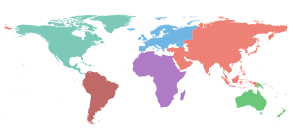
\includegraphics[scale=0.3]{img/map.png} \\
      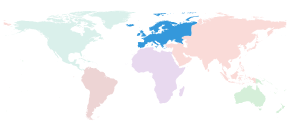
\includegraphics[scale=0.3]{img/map_selected.png}
    \end{figure}
  \end{column}
\end{columns}
\begin{itemize}
\item Choice of color : 
\item Rectangular projection : Most used projection  
\end{itemize}
\end{frame}

\begin{frame}
\frametitle{Design - Nutriscore Bar Chart}
\begin{columns}[T]
  \begin{column}{.7\textwidth}
    \begin{table}
      \resizebox{1.0\textwidth}{!}{
        \centering
      \begin{tabular}{|c|c|c|c||c|c|c|c|c|c|c||c|}
        \hline
        Name & D & F & D' & X & Y & Z & T & R & \_ & [] & CP\\
        \hline\hline
        Grade & O & > &  & A &  & &  & C & &  & \\
        \hline
        Number of product & Q & > &  &  & A &  &  & S &  &  & \\
        \hline
      \end{tabular}
    }
    \end{table}
  \end{column}
  \begin{column}{.25\textwidth}
    \begin{figure}
      \centering
      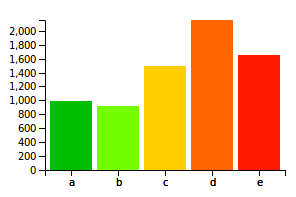
\includegraphics[scale=0.3]{img/nutriscore.png}
    \end{figure}
  \end{column}
\end{columns}
\begin{itemize}
\item Choice of color : color used for nutriscore

\includegraphics[scale=0.2]{img/nutri-score.jpg} 
\end{itemize}
\end{frame}

\begin{frame}
\frametitle{Design - Categories Pie Chart}

\begin{columns}[T]
  \begin{column}{.7\textwidth}
    \begin{table}
      \resizebox{1.0\textwidth}{!}{
        \centering
      \begin{tabular}{|c|c|c|c||c|c|c|c|c|c|c||c|}
        \hline
        Name & D & F & D' & X & Y & Z & T & R & \_ & [] & CP\\
        \hline\hline
        Categorie & N & f &  & A & A &  &  & T &  &  & \\
        \hline
        Number of product  & N & f &  & A & A &  &  & S,V &  &  & \\
        \hline
      \end{tabular}
    }
    \end{table}
  \end{column}
  \begin{column}{.25\textwidth}
    \begin{figure}
      \centering
      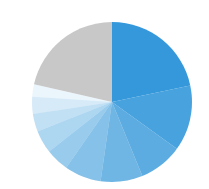
\includegraphics[scale=0.3]{img/piechart.png}
    \end{figure}
  \end{column}
\end{columns}
\end{frame}

\begin{frame}
\frametitle{Design - Country Chart}

\begin{columns}[T]
  \begin{column}{.7\textwidth}
    \begin{table}
      \resizebox{1.0\textwidth}{!}{
        \centering
      \begin{tabular}{|c|c|c|c||c|c|c|c|c|c|c||c|}
        \hline
        Name & D & F & D' & X & Y & Z & T & R & \_ & [] & CP\\
        \hline\hline
        Country & N & f &  & P  &  P &  &  & T &  &  & \\
        \hline
        Continent & N & f &  &  &  &  &  & C &  &  & \\
        \hline
        Number of products & Q & > &  &P  &  &  &  & &  &  & \\
        \hline
        Number of categories & Q & > &  &  &P  &  &  & &  &  & \\
        \hline
        Proportion of grade A products & Q & > &  &  &  &  &  & S &  &  & \\
        \hline
      \end{tabular}
    }
    \end{table}
  \end{column}
  \begin{column}{.25\textwidth}
    \begin{figure}
      \centering
      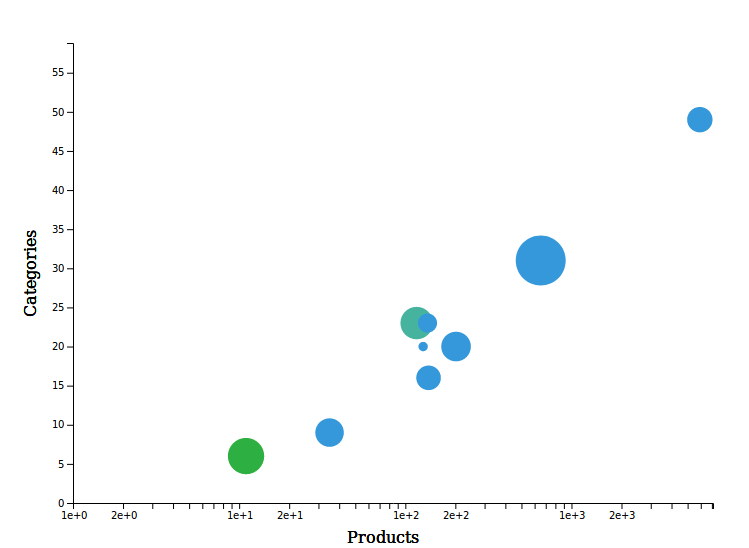
\includegraphics[scale=0.1]{img/country.png}
    \end{figure}
  \end{column}
\end{columns}
\begin{itemize}
\item Log Scale for X Axis : Smooth curve 
\end{itemize}
\end{frame}

\section{Demonstration}
\begin{frame}
  \frametitle{Demonstration}
\end{frame}
\end{document}
